\section{PS4b: StringSound}\label{sec:ps4b}

\subsection{Discussion}\label{sec:ps4b:disc}

This project uses the Karplus-Strong algorithm to simulate the plucking of a guitar, CircularBuffer.hpp that I made for ps4a to store the keys and notes. Therefore, you keyboard become a piano.

\begin{figure}[tbh]
	\centering
	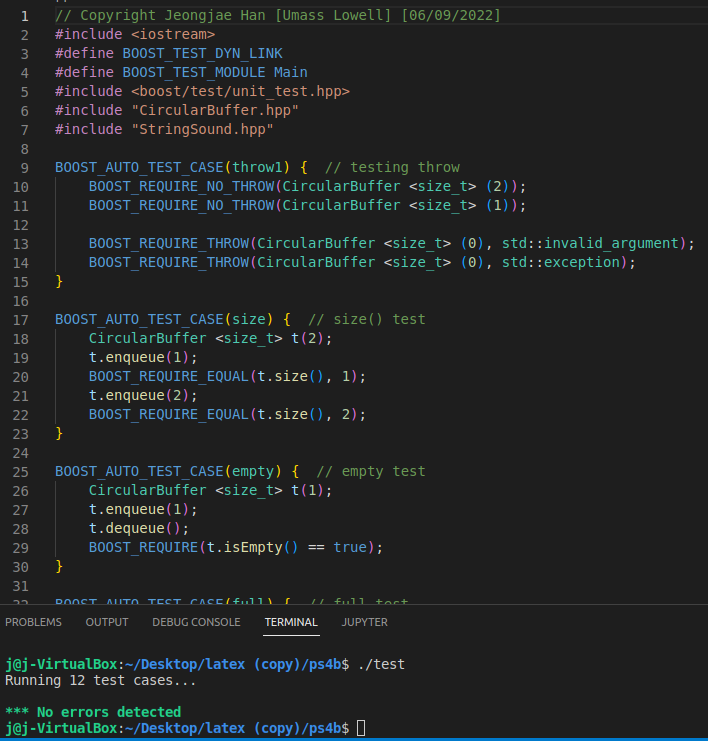
\includegraphics[width=8cm]{ps4b_test}
	\caption{Testing the hpp, and cpp of this project}
	\label{fig:ps4b_test}
\end{figure}

I wrote the tests for all the public functions: Constructors, pluck, time, tic, and sample. I constructor to throw invalid-argument exception when the user tries to put invalid-argument. Other fuctions passed the test.

\begin{figure}[tbh]
	\centering
	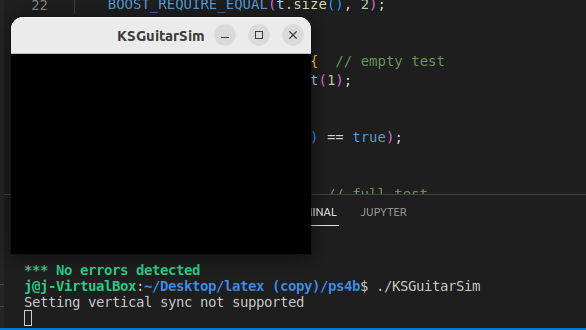
\includegraphics[width=10cm]{ps4b}
	\caption{The window of KSGuitarSim it runs as it should}
	\label{fig:ps4b}
\end{figure}

Cannot put audio on this file, so I cannot prove that the program makes right sound, but I want to show that when you run it it will show black window. 

\subsection{Places to get help}

Lecture slide to understand the calculation and physics.
cppreference

%\subsection{What I accomplished}\label{sec:ps0:accomplish}

%\subsection{What I already knew}\label{sec:ps0:knew}

%\subsection{What I learned}\label{sec:ps0:learned}

\subsection{Challenges}\label{sec:ps4b:challenges}

Instead of switch, I made the program finds and recognizes the input and finds the right note.
For the lambda expression, I tried the template on the lecture slide, but it was not working. Therefore, I googled it and cppreference showed me different ways to use it and found a syntax that works for this.

\subsection{Mistakes}\label{sec:ps4b:Mistakes}

I got 0.5 points off because I used lambda for Karplus-Strong algorithm. In order to get the return value of tick, I needed to use the average of two items that are stored in CircularBuffer and multiply by decay rate. I used the lambda to get average of two items. I did not use any algorithm functions because it was easier to code by myself. However, I had to call lambda by passing it as an argument, but the way I used was calling lambda directly.

\subsection{Codebase}\label{sec:ps4b:code}
Makefile
\lstinputlisting[language=Make]{ps4b/Makefile}
KSGuitarSim.cpp
\lstinputlisting{ps4b/KSGuitarSim.cpp}
CircularBuffer.hpp
\lstinputlisting{ps4b/CircularBuffer.hpp}
StringSound.hpp
\lstinputlisting{ps4b/StringSound.hpp}
StringSound.cpp
\lstinputlisting{ps4b/StringSound.cpp}
test.cpp
\lstinputlisting{ps4b/test.cpp}

\newpage
